\documentclass[10pt,twocolumn,letterpaper]{article}
%\usepackage[top=0.75in,bottom=1in,left=0.75in,right=0.75in,columnsep=0.25in,headheight=10pt,headsep=10pt,footskip=25pt]{geometry}
\usepackage[letterpaper,textwidth=6.75in,textheight=9.0in,left=0.77in,top=0.75in,columnsep=0.25in,headheight=10pt,headsep=10pt,footskip=25pt]{geometry}
\usepackage{times}
\usepackage{natbib}
% Shared preamble for ICML and arXiv versions

\usepackage{amsmath}
\usepackage{amssymb}
\usepackage{booktabs}
\usepackage{graphicx}
\usepackage{microtype}
\usepackage{enumitem}
\setlist{nosep,leftmargin=*}

% Algorithms
\usepackage{algorithm}
\usepackage{algorithmic}
\renewcommand{\algorithmicdo}{}
\renewcommand{\algorithmicendfor}{\textbf{end}}
\renewcommand{\algorithmicendif}{\textbf{end}}
\newcommand{\LCOMMENT}[1]{\hfill\textit{\# #1}}

% TikZ
\usepackage{tikz}
\usepackage{pgfplots}
\pgfplotsset{compat=1.18}
\usetikzlibrary{arrows.meta,positioning}

% Colors
\definecolor{DarkBlue}{RGB}{51,102,204}
\definecolor{LightBlue}{RGB}{102,178,255}
\definecolor{DarkRed}{RGB}{153,0,51}
\definecolor{LightPurple}{RGB}{204,153,255}
\definecolor{Purple}{RGB}{128,0,128}
\definecolor{LinkBlue}{RGB}{0,0,139}

% Hyperref and cleveref (must be last)
\usepackage[breaklinks=true,bookmarks=false,colorlinks=true,linkcolor=LinkBlue,citecolor=LinkBlue,urlcolor=LinkBlue]{hyperref}
\usepackage[capitalize,noabbrev]{cleveref}


\renewcommand{\L}{\mathcal{L}}
\newcommand{\X}{\mathcal{X}}
\newcommand{\Y}{\mathcal{Y}}
\newcommand{\Z}{\mathcal{Z}}

\renewcommand{\H}{\operatorname{\mathsf H}}
\newcommand{\I}{\operatorname{\mathsf I}}
\newcommand{\K}{\operatorname{\mathsf K}}
\newcommand{\E}{\operatorname{\mathsf E}}
\newcommand{\D}{\operatorname{\mathsf D}}
\newcommand{\F}{\operatorname{\mathsf{F}}}

\newcommand{\dd}{\mathrm{d}}

\newcommand{\bilinear}{\operatorname{Bilinear}}

\newcommand{\softmax}{\operatorname{softmax}}
\newcommand{\sigmoid}{\operatorname{sigmoid}}
\newcommand{\expit}{\operatorname{expit}}
\newcommand{\logit}{\operatorname{logit}}

\newcommand{\reals}{\mathbb{R}}
\newcommand{\ints}{\mathbb{Z}}
\newcommand{\simplex}{\mathbb{P}}

\newcommand\scalemath[2]{\scalebox{#1}{\mbox{\ensuremath{\displaystyle #2}}}}
\newcommand{\defeq}{\stackrel{\scalemath{0.5}{\mathrm{def}}}{=}}
\newcommand{\iid}{\stackrel{\scalemath{0.5}{\mathrm{iid}}}{\sim}}
\newcommand{\tee}{{\scalemath{0.5}{\mathsf{T}}}}

\newcommand{\Bernoulli}{\operatorname{Bernoulli}}
\newcommand{\Categorical}{\operatorname{Categorical}}
\newcommand{\Poisson}{\operatorname{Poisson}}
\newcommand{\MVN}{\operatorname{MVN}}
\newcommand{\Uniform}{\operatorname{Uniform}}

\newcommand{\snr}{\mathrm{SNR}}

\newcommand{\for}{\mathrm{for}\;\;}
\renewcommand{\stop}{\operatorname{stop}}
\newcommand{\size}{\operatorname{size}}

\newcommand{\argmin}{\operatornamewithlimits{arg\, min}}
\newcommand{\argmax}{\operatornamewithlimits{arg\, max}}

\newcommand{\of}{\circ}
\newcommand{\distance}{\operatorname{distance}}

\newcommand{\reshape}{\operatorname{reshape}}
\newcommand{\transpose}{\operatorname{transpose}}
\newcommand{\rearrange}{\operatorname{rearrange}}
\newcommand{\shape}{\operatorname{shape}}
\newcommand{\ndims}{\operatorname{ndims}}

\newcommand{\Encoder}{\operatorname{Encoder}}
\newcommand{\Decoder}{\operatorname{Decoder}}


% Default fixed font does not support bold face
\DeclareFixedFont{\ttb}{T1}{txtt}{bx}{n}{10} % for bold
\DeclareFixedFont{\ttm}{T1}{txtt}{m}{n}{10}  % for normal

% Custom colors
\usepackage{color}
\definecolor{deepblue}{rgb}{0,0,0.5}
\definecolor{deepred}{rgb}{0.6,0,0}
\definecolor{deepgreen}{rgb}{0,0.5,0}

\usepackage{listings}

% Python style for highlighting
%\newcommand\pythonstyle{\lstset{
%language=Python,
%basicstyle=\ttm,
%morekeywords={self},              % Add keywords here
%keywordstyle=\ttb\color{deepblue},
%emph={MyClass,__init__},          % Custom highlighting
%emphstyle=\ttb\color{deepred},    % Custom highlighting style
%stringstyle=\color{deepgreen},
%frame=tb,                         % Any extra options here
%showstringspaces=false
%}}

\newcommand\pythonstyle{\lstset{
language=Python,
basicstyle=\footnotesize\ttm,
keywordstyle=\ttb\color{deepblue},
commentstyle=\ttm\color{deepgreen},
stringstyle=\color{deeporange},
emphstyle=\ttb\color{deepred},    % Custom highlighting style.
emph={__init__,__call__},          % Custom highlighting.
otherkeywords={self,yield},       % Additional keywords.
frame=single,                     % `tb` for top-bottom, `single` for square.
showstringspaces=false,
breaklines=true,
backgroundcolor=\color{verylightgray},
}}

% Python environment
\lstnewenvironment{python}[1][]
{
\pythonstyle
\lstset{#1}
}
{}

% Python for inline
\newcommand\pythoninline[1]{{\pythonstyle\lstinline!#1!}}
\renewcommand{\v}[1]{\pythoninline{#1}}

% Python for external files
\newcommand\pythonexternal[2][]{{
\pythonstyle
\lstinputlisting[#1]{#2}}}

%\usepackage[ruled,vlined]{algorithm2e}


% No paragraph indent, use vertical space instead.
\setlength{\parindent}{0pt}
\setlength{\parskip}{6pt}

% Slightly tighter section spacing.
\makeatletter
\renewcommand\section{\@startsection{section}{1}{\z@}{-0.12in}{0.02in}{\normalfont\large\bfseries}}
\renewcommand\subsection{\@startsection{subsection}{2}{\z@}{-0.10in}{0.01in}{\normalfont\normalsize\bfseries}}
\renewcommand\subsubsection{\@startsection{subsubsection}{3}{\z@}{-0.08in}{0.01in}{\normalfont\normalsize\bfseries}}

% Title with horizontal rules.
\def\@maketitle{%
  \hrule height1pt \vskip .35in
  \begin{center}%
    {\Large\bfseries \@title \par}%
    \vskip 1em%
    {\normalsize \@author \par}%
  \end{center}%
  \vskip 0in \hrule height1pt \vskip .2in}
\makeatother

% Centered abstract title, slightly narrower.
\renewenvironment{abstract}{\centerline{\large\bfseries Abstract}\vspace{-0.12in}\begin{quote}}{\par\end{quote}\vskip 0.12in}

% Running header with title on pages 2+.
\usepackage{fancyhdr}
\pagestyle{fancy}
\fancyhf{}
\fancyhead[C]{\small\bfseries Speed is Confidence}
\fancyfoot[C]{\thepage}
\renewcommand{\headrulewidth}{1pt}
\fancypagestyle{plain}{\fancyhf{}\fancyfoot[C]{\thepage}\renewcommand{\headrulewidth}{0pt}} % first page: no header

\title{\vspace{-1em}Speed is Confidence\vspace{-0.5em}}
\author{Joshua V.\ Dillon\\Independent Researcher\\\tt\small \href{mailto:jvdillon@gmail.com}{jvdillon@gmail.com}}
\date{\vspace{-2em}}

\begin{document}

%\twocolumn[
\maketitle
\begin{abstract}
%\setlength{\parskip}{6pt}
Biological neural systems must be fast but are energy-constrained. Evolution's solution: act on the first signal. Winner-take-all circuits and time-to-first-spike coding implicitly treat \emph{when} a neuron fires as an expression of confidence.

% Sources:
%   97.2% halt-first: x02.log, x03.log, x04.log (3 seeds × 4 rotations)
%   86.1% baseline: x00.log (unfuck.txt)
%   97.3% TTA: x00.log with 8 rotations (unfuck.txt)
We apply this principle to ensembles of Tiny Recursive Models (TRM)~\citep{jolicoeur2025trm}. By basing the ensemble prediction solely on the first to halt rather than averaging predictions, we achieve 97.2\% puzzle accuracy on Sudoku-Extreme while using 10$\times$ less compute than test-time augmentation (the baseline achieves 86.1\% single-pass, 97.3\% with TTA). Inference speed is an implicit indication of confidence.

% Source: x182{a,b,c,d}.log (randn): 96.85% ± 0.58%
But can this capability be manifested as a training-only cost? Evidently yes: by maintaining $K{=}4$ parallel latent states during training but backpropping only through the lowest-loss ``winner,'' a single model achieves \textbf{96.9\% $\pm$ 0.6\%} puzzle accuracy---roughly matching TTA performance without any test-time augmentation.

As in nature, this work was also resource constrained: all experimentation used a single RTX 5090. This necessitated efficiency and compelled our invention of a modified SwiGLU~\citep{shazeer2020swiglu} which made Muon~\citep{jordan2024muon} viable. With these improvements and $K{=}1$ training, we match TRM baseline performance ($\sim$87\%) in just 48 min (8k steps, bs${=}$384, ${\sim}$16GiB). Higher accuracy ($\sim$97\%) is achieved in 36k steps and $K{=}4$ (bs${=}$192, ${\sim}$30GiB) and takes about 6 hours.

% The path: biological principle $\to$ inference strategy that validates it $\to$ training procedure that internalizes the benefit. Speed is confidence.

Code: \url{https://github.com/jvdillon/sic}
\end{abstract}
%\vspace{0.5cm}
%]

\section{Introduction}

When faced with uncertainty, biological neural systems don't deliberate
indefinitely---they act on the first confident signal. This principle, refined
by millions of years of evolution, underlies rapid decision-making from prey
detection to social judgment. In cortical winner-take-all circuits, competing
neural populations race to threshold; the first to fire suppresses alternatives
and triggers action~\citep{grossberg1987competitive}. The speed of convergence
itself carries information: a fast response indicates a clear, unambiguous
stimulus.

We apply this biological insight to improve neural network ensembles. Standard
ensemble methods average predictions across models, treating all outputs
equally regardless of when each model reaches its answer. For iterative
reasoners with adaptive computation time (ACT)~\citep{graves2016act}, this
discards valuable information: models that converge quickly have typically
found ``clean'' solution paths, while those still deliberating are often stuck
or uncertain.

Our key observation is that \textbf{inference speed is an implicit confidence
signal}. When multiple models reason in parallel, the first to halt is most
likely correct. This simple selection rule---which we call \emph{halt-first
ensembling}---improves accuracy by 5.7 percentage points over probability
averaging while using 10$\times$ less compute on the Sudoku-Extreme benchmark.

This raises a natural question: can we internalize this benefit within a single
model? Training and deploying multiple models is expensive. We show that the
diversity exploited by halt-first selection comes primarily from different
random initializations during training. By maintaining $K$ parallel latent
initializations within one model and training with a winner-take-all (WTA)
objective, we achieve ensemble-level accuracy with single-model deployment
cost.

\paragraph{Contributions.}
\begin{enumerate}
  \item We demonstrate that halt-first selection outperforms probability
    averaging for ensembles of iterative reasoners, achieving 97.2\% accuracy
    vs.\ 91.5\% with 10$\times$ less compute.
  \item We introduce \emph{oracle-first training}, a WTA method that
    internalizes ensemble diversity within a single model, achieving
    96.9\% $\pm$ 0.6\% accuracy with zero inference overhead.
  \item We identify chain convergence during training and introduce
    \emph{expunging}---removing converged hypotheses to recover compute for
    new samples.
  \item We discover that Muon optimization fails with standard SwiGLU and
    provide a fix: layer normalization before the down-projection. This
    enables 4$\times$ higher learning rates than AdamW.
  \item We provide a theoretical interpretation connecting halting speed to
    the spectral properties of bilevel equilibria, grounding ``speed is
    confidence'' in the conditioning of nested fixed points.
  \item We document extensive hyperparameter exploration across 180+
    experiments, identifying critical factors: carry policy, SVD-aligned
    initialization, and z\_L diversity. Code and trained models at
    \url{https://anonymous.4open.science/r/TODO}.
\end{enumerate}

% NARRATIVE: Establish the technical foundation. Reader needs to understand TRM
% and ACT before we can explain halt-first selection and oracle-first training.
\section{Background}

\subsection{Tiny Recursive Models}

Tiny Recursive Models (TRM)~\citep{jolicoeur2025trm} achieve strong performance
on constraint satisfaction problems using a remarkably simple architecture: a
small neural network that iteratively refines its predictions through recursive
application:
%
\begin{algorithm}[h]
\caption{TRM with ACT (Inference)}
\label{alg:trm}
\begin{algorithmic}[1]
  \FOR{$t = 0, \ldots, n_\text{ACT}{-}1$ \LCOMMENT{$n_\text{ACT}{=}16$}}
    \FOR{$i = 0, \ldots, n_\text{H}{-}1$ \LCOMMENT{$n_\text{H}{=}6$}}
      \STATE $z_L, z_H \gets \operatorname{stop}(z_L), \operatorname{stop}(z_H)$
      \FOR{$j = 0, \ldots, n_\text{L}{-}1$ \LCOMMENT{$n_\text{L}{=}9$}}
        \STATE $z_L \gets f(\operatorname{embed}(x;\theta) + z_L + z_H;\theta)$
      \ENDFOR
      \STATE $z_H \gets f(z_L + z_H;\theta)$
    \ENDFOR
    \STATE $y,q \gets h_\text{puzzle}(z_H;\theta), h_\text{halt}(z_H;\theta)$
    \IF{$q > 0$}
      \STATE \textbf{break}
    \ENDIF
  \ENDFOR
\end{algorithmic}
\end{algorithm}
%
The model maintains two latent states: $z_L$ for ``low-level'' details (updated
$n_\text{L}$ times per H-cycle, i.e., one outer loop iteration) and $z_H$ for
``high-level'' reasoning (updated once per H-cycle). The $\operatorname{stop}(\cdot)$ operator detaches
its argument from the computation graph, preventing gradient flow between
H-cycles and enabling stable training.

On Sudoku-Extreme (17-clue puzzles, the minimum for uniqueness), a 7M parameter
TRM achieves ${\sim}$86\% puzzle accuracy---substantially outperforming larger
language models while using a fraction of the parameters.

\subsection{Adaptive Computation Time}

Rather than fixing the number of iterations $T$, TRM can learn \emph{when to
stop} via Adaptive Computation Time (ACT)~\citep{graves2016act}. The model
outputs a halting probability $q_\text{halt}\defeq\sigmoid(q)$ at each step,
trained to predict whether the current output is correct. When $q_\text{halt} >
0.5$, the model ``commits'' to its answer.

This creates an implicit tradeoff: easy puzzles should halt quickly (high
confidence after few iterations), while hard puzzles may require more
computation. In practice, a well-trained TRM solves most Sudoku puzzles in 1--3
steps, with a long tail requiring up to 16 iterations.

\section{Method}

\subsection{The Ensemble Puzzle}

Standard practice for improving accuracy is
ensembling~\citep{dietterich2000ensemble}: train multiple models with different
seeds and average their predictions. For TRM on Sudoku-Extreme:
%
% Source: x02.log (86.02%), x03.log (83.87%), x04.log (85.03%) - noised models
\begin{center}
\begin{tabular}{lcc}
\toprule
Method & Puzzle Acc. & Forward Passes \\
\midrule
Single model & 84.97\% & 16 \\  % avg(x02.log, x03.log, x04.log)
Ensemble (3 seeds) & 88.52\% & 48 \\  % x02.log + x03.log + x04.log
+ TTA (4 rotations) & 91.51\% & 192 \\  % x02.log + x03.log + x04.log + TTA
\bottomrule
\end{tabular}
\end{center}
%
Ensemble plus test-time augmentation yields +6.5\% accuracy, but at
12$\times$ the compute cost. This presents a puzzle: ensembling helps, but the
standard approach of probability averaging seems wasteful. Each model in the
ensemble has its own ``opinion'' about when to stop reasoning, yet we ignore
this timing information entirely. Can we do better by paying attention to
\emph{when} models commit to their answers?

We begin with a biological intuition and follow it to its logical conclusion.

Biological neural systems face a fundamental constraint: metabolic energy is
scarce, yet decisions must be fast. Evolution's solution is to \emph{act on
the first confident signal}. In cortical winner-take-all
circuits~\citep{grossberg1987competitive}, competing neural populations race to
threshold, with the first to fire suppressing alternatives. Spiking neural
networks formalize this as time-to-first-spike (TTFS)
coding~\citep{thorpe2001spike, park2020t2fsnn}, where information is encoded in
\emph{when} neurons fire rather than \emph{how often}---achieving both speed
and energy efficiency.

This principle suggests a strategy for ensembles of iterative reasoners:
instead of averaging probabilities, \textbf{select the first model to halt}.

\subsection{Halt-First Ensemble}

The procedure is simple: run all ensemble members in parallel, each performing
its own ACT iterations. When any model's halting signal exceeds threshold, that
model provides the final answer. The results are striking:
%
% Source: x02.log, x03.log, x04.log (3 seeds × 4 rotations = 12 chains)
\begin{center}
\begin{tabular}{@{}lccc@{}}
\toprule
Method & Acc. & Steps & Speedup \\
\midrule
Prob.\ avg.\ (12) & 91.5\% & 192 & 1$\times$ \\  % x02.log + x03.log + x04.log + TTA
\textbf{Halt-first (12)} & \textbf{97.2\%} & \textbf{18.5} & \textbf{10$\times$} \\  % x02.log + x03.log + x04.log + TTA halt-first
\bottomrule
\end{tabular}
\end{center}
%
Halt-first selection improves accuracy by 5.7 percentage points while using
10$\times$ less compute. This validates the biological intuition:
\textbf{inference speed is an implicit confidence signal}. When a reasoning
process converges quickly, it indicates the model has found a ``clean''
solution path---one without contradictions or backtracking. Probability
averaging destroys this signal; halt-first selection preserves the information
that evolution discovered: the reasoner that finishes first is most likely
correct. We analyze the halting dynamics in detail in \Cref{sec:halting}.

\subsection{Oracle-First Training}

The halt-first result raises a natural question: can we internalize this
benefit within a single model? Deploying multiple models is expensive---we want
the accuracy of an ensemble with the deployment cost of one.

Our key insight is that ensemble diversity comes from different random
initializations during training. We can internalize this diversity by
maintaining $K$ parallel latent initializations \emph{within} one model and
letting them compete. During training, we run $K{=}4$ parallel hypotheses; at
inference, we run just one.

Specifically, we maintain $K$ parallel low-level states
$\{z_L^{(k)}\}_{k=1}^K$, each from a learned initialization
$L_{\text{init}}^{(k)}$, while sharing the high-level state $z_H$. At each
step, all $K$ heads process the input in parallel, and the
\textbf{winner-take-all} (WTA) rule selects which head receives the gradient:
%
\begin{equation}
  k^* = \argmin_k \mathcal{L}(y^{(k)}, y_\text{target})
\end{equation}
%
Only the winning head contributes to the loss. This mirrors halt-first
selection: at inference, the fastest model wins; during training, the most
accurate head wins. Both reward the same underlying property: having found a
clean solution path. The connection is deep---we are teaching the model to find
confident solutions by making confidence (low loss) the criterion for receiving
gradient signal.

\paragraph{Training dynamics.} A key detail: TRM training ``unpacks'' the outer
loop of \Cref{alg:trm}. Each gradient step performs one H-cycle, carrying
$z_H$ and $z_L$ to the next step. This means the $K$ parallel chains evolve
across multiple gradient updates, not within a single forward pass.

\paragraph{Carry policy.} After each step, we must decide how to propagate
states to the next iteration. We use \texttt{copy\_top1} for $z_H$: the
winner's $z_H$ is copied to all chains (\Cref{alg:wta}, line 8). For $z_L$, we
use \texttt{all}: each chain keeps its own $z_L$. This allows heads to benefit
from shared high-level progress while maintaining low-level diversity (see
\Cref{sec:ablations} for ablations).

\begin{algorithm}[h]
\caption{Oracle-First Training (one step)}
\label{alg:wta}
\begin{algorithmic}[1]
  \STATE \textbf{Input:} $x$, $y_\text{target}$, carried $z_H$, $\{z_L^{(k)}\}_{k=1}^K$
  \FOR{$k = 1$ to $K$}
    \STATE $y_k, q_k, z_H', z_L^{(k)} \gets \operatorname{TRM}(x, z_H, z_L^{(k)}; \theta)$
  \ENDFOR
  \STATE $k^* \gets \argmin_{k} \mathcal{L}_\text{CE}(y_k, y_\text{target})$ \LCOMMENT{winner}
  \STATE $c \gets \mathbf{1}[y_{k^*} = y_\text{target}]$ \LCOMMENT{correctness}
  \STATE $\mathcal{L} \gets \mathcal{L}_\text{CE}(y_{k^*}, y_\text{target}) + \lambda \mathcal{L}_\text{BCE}(\sigma(q_{k^*}), c)$
  \STATE Backprop through $\mathcal{L}$
  \STATE $z_H \gets z_H'$ \LCOMMENT{winner's $z_H$ shared to all}
\end{algorithmic}
\end{algorithm}
%
\noindent Here $\mathcal{L}_\text{CE}$ is cross-entropy with label smoothing
($\alpha{=}0.2$), $\mathcal{L}_\text{BCE}$ is binary cross-entropy for the
halting signal where $q_k$ is the halting logit and $\sigma(q_k)$ is the
halting probability, and $\lambda{=}0.05$.

\paragraph{Counter-intuitive design.} WTA training deliberately spends compute
on reasoning chains that won't contribute to the gradient. This apparent waste
enables exploration: losing heads probe alternative paths, and winner selection
identifies which succeeded.

\subsection{Faster Training}

WTA training requires $K$ forward passes per iteration---a $4\times$ increase
for $K{=}4$. With only a single GPU, efficient training is essential. We
combine two techniques that reduce training time from days to hours, making
rapid experimentation possible.

\subsubsection{Muon Optimizer}

We use Muon~\citep{jordan2024muon} for 2D weight matrices (lr${=}$0.02,
wd${=}$0.005) and AdamW for embeddings, heads, and biases (lr${=}10^{-4}$,
wd${=}$1.0, $\beta{=}$(0.9, 0.95)). Muon's orthogonalized momentum enables
substantially higher learning rates than AdamW alone, accelerating convergence.
However, Muon is magnitude-invariant, so bias-like parameters require AdamW.
Learning rate follows a cosine schedule.

\paragraph{Selective regularization.} This split-optimizer design creates an
asymmetric regularization structure: the core reasoning weights (MLPMixer
blocks) receive minimal regularization via Muon's low weight decay, while
embeddings and output heads receive strong regularization via AdamW's high
weight decay. Combined with label smoothing ($\alpha{=}0.2$), this encourages
the core model to learn expressive representations while preventing the
input/output interfaces from overfitting. In contrast, baseline TRM applies
uniform high weight decay (1.0) to all parameters, which may over-constrain
the reasoning layers.

\paragraph{Modified SwiGLU.} We discovered that Muon fails completely with
standard SwiGLU activation. The fix is to apply layer normalization before the
down-projection: $\text{SwiGLU}_\text{mod}(x) = \text{SiLU}(g) \cdot
\text{LayerNorm}(g \odot x)$ where $g = Wx$. Without this modification, Muon's
orthogonalized updates cause training to diverge.

\subsubsection{SVD-Aligned Initialization}

The $K$ initialization vectors $L_{\text{init}}^{(k)}$ determine hypothesis
diversity. Naive random initialization risks ``dead'' heads---initializations
that point in directions the network cannot use effectively. We address this by
computing the top singular vectors of the first layer's weight matrix and
ensuring all $K$ heads have equal alignment with this subspace. This provides
equal ``effective signal strength'' across heads while maintaining diversity in
the orthogonal complement.

\subsection{Intuition: Why Speed Indicates Confidence}

We offer a speculative interpretation connecting halting speed to optimization
conditioning. This is a hypothesis, not a formal result; empirical validation
is future work.

\paragraph{Bilevel fixed-point structure.} TRM computes a nested equilibrium:
%
\begin{align}
  z_L^* &= f(z_L^*, z_H, z_x) && \text{(inner: fast local refinement)} \\
  z_H^* &= g(z_H^*, z_L^*) && \text{(outer: slow global integration)}
\end{align}
%
The inner loop equilibrates $z_L$ for fixed $z_H$; the outer loop updates $z_H$
given the equilibrated $z_L^*$. This separation creates a natural hierarchy:
$z_L$ handles cell-level constraint propagation while $z_H$ maintains
puzzle-level state.

\paragraph{Architectural asymmetry stabilizes the inner loop.} A key
observation: $z_x$, $z_L$, and $z_H$ each have unit variance (due to
normalization), but they enter the computation asymmetrically. L-cycles receive
$z_L + z_H + z_x$ (three terms), while H-cycles receive only $z_H + z_L$ (two
terms). Assuming approximate independence, $z_L$ contributes $\tfrac{1}{3}$ of
L-cycle input variance versus $\tfrac{1}{2}$ for H-cycles.

The Jacobian $J_L = \partial f / \partial z_L$ measures sensitivity to $z_L$
perturbations. When $z_L$ is a smaller fraction of the input, the output is
more ``anchored'' by context $(z_H + z_x)$ and less sensitive to $z_L$---yielding
smaller spectral radius. The fixed input $z_x$ thus acts as a stabilizing
anchor that L-cycles have but H-cycles lack, naturally making the inner loop
better conditioned than the outer loop.

\paragraph{WTA training enhances this effect.} The \texttt{copy\_top1} carry
policy (\Cref{alg:wta}, line~8) copies the winner's $z_H$ to all chains. This
means each chain's $z_H$ comes from a \emph{different} chain than its $z_L$,
further decorrelating the inputs and strengthening the independence assumption
underlying the variance argument.

\paragraph{Speed reflects conditioning (conjecture).} For iterative fixed-point
methods, convergence rate depends on the spectral radius of the iteration
Jacobian---smaller spectral radius means faster convergence. We hypothesize
that the learned halting signal $q_\text{halt}$ correlates with this
conditioning: chains that halt quickly have found well-conditioned paths, while
chains that deliberate longer are stuck in poorly-conditioned regions.
Evolution's heuristic (trust the first signal) may thus correspond to selecting
well-conditioned solutions.

\section{Related Work}

\paragraph{Recursive reasoning models.}
Tiny Recursive Models (TRM)~\citep{jolicoeur2025trm} demonstrate that small
networks with iterative refinement can outperform larger models on constraint
satisfaction. The key insight is that recursive application of a small network
can implement complex reasoning through gradual refinement, similar to how
iterative algorithms solve constraint satisfaction problems. Our work extends
TRM with multi-head stochastic search, showing that the diversity lost by using
a single model can be recovered through parallel latent initializations. Deep
Improvement Supervision~\citep{dis2025} takes a different approach, providing
explicit intermediate targets rather than relying on implicit refinement; this
is complementary to our winner-take-all dynamics.

\paragraph{Adaptive computation.}
Adaptive Computation Time (ACT)~\citep{graves2016act} allows models to learn
when to stop iterating. PonderNet~\citep{banino2021pondernet} reformulates
halting as a probabilistic model with unbiased gradients. Universal
Transformers~\citep{dehghani2018universal} apply depth-adaptive computation to
transformers. Our key observation is that the halting signal encodes
confidence, making first-to-halt selection superior to probability averaging.

\paragraph{Early-exit ensembles.}
Recent work shows that \emph{cascaded} ensembles with early exit can be more
efficient than scaling single models~\citep{xia2023earlyexit}. These approaches
run ensemble members \emph{sequentially}, exiting when confidence exceeds a
threshold. Our halt-first selection differs fundamentally: we run models
\emph{in parallel} and select whichever halts first. This exploits timing as a
confidence signal rather than explicit confidence scores, and achieves both
higher accuracy and lower latency than sequential cascades.

\paragraph{Dynamic ensemble selection.}
Dynamic Ensemble Selection (DES)~\citep{cruz2018deslib} chooses which model to
use based on input features, using $k$-nearest neighbors to identify locally
competent classifiers. This requires explicit competence estimation; our
approach needs no such mechanism---halting time implicitly identifies the most
confident model.

\paragraph{Portfolio solvers.}
In constraint satisfaction, algorithm portfolios~\citep{gomes2001satportfolio}
run multiple solvers in parallel, terminating when any solver
succeeds~\citep{luby1993optimal}. This ``first to finish'' strategy is optimal
for Las Vegas algorithms where run times are unpredictable. Our halt-first
ensemble applies this principle to neural iterative reasoners---to our
knowledge, the first such application. The key insight is that ACT-style
halting provides a natural ``finish'' signal analogous to solver termination.

\paragraph{Diverse solution strategies.}
PolyNet~\citep{hottung2025polynet} learns multiple complementary solution
strategies within a single decoder for combinatorial optimization, allowing
different strategies to specialize on different problem subsets. Our approach
shares the goal of implicit diversity but differs in mechanism: PolyNet learns
diverse \emph{construction policies}, while we maintain diverse \emph{latent
initializations} that compete via winner-take-all dynamics. PolyNet selects
strategies via explicit scoring; we select via oracle (training) or halting
time (inference).

\paragraph{Winner-take-all and competitive learning.}
WTA dynamics appear in competitive learning~\citep{rumelhart1985competitive},
mixture of experts~\citep{shazeer2017moe}, and sparse
attention~\citep{child2019sparse}. Our use of WTA differs: we apply it to
\emph{latent initializations} rather than network components, creating
competition among reasoning trajectories rather than experts.

\paragraph{Test-time compute scaling.}
Recent work explores scaling compute at inference time rather than model size.
Chain-of-thought prompting, tree search, and iterative refinement all trade
inference compute for accuracy. Our work contributes to this paradigm: halt-first
selection achieves \emph{better} accuracy with \emph{less} compute by
exploiting the structure of iterative reasoning. Rather than uniformly
allocating compute across all inputs, we let the model adaptively allocate
based on difficulty---easy puzzles halt immediately, hard puzzles iterate
longer. WTA training goes further, internalizing this adaptive compute
allocation within a single model.

\paragraph{Biological inspiration.}
Time-to-first-spike (TTFS) coding in spiking neural
networks~\citep{thorpe2001spike, park2020t2fsnn} encodes information in
\emph{when} neurons fire rather than firing rates, achieving both speed and
energy efficiency. Winner-take-all circuits in cortex suppress alternatives
once a threshold is reached~\citep{grossberg1987competitive}. At a higher
organizational level, the Thousand Brains
theory~\citep{hawkins2021thousand} proposes that cortical columns operate as
parallel models that vote to reach consensus. Our halt-first ensemble embodies
these principles: parallel reasoners race, and the first to ``fire'' (halt)
provides the answer. Human decision-making shows analogous speed-accuracy
tradeoffs~\citep{heitz2014speedaccuracy}, formalized in drift-diffusion
models~\citep{ratcliff2008diffusion} as evidence accumulation until threshold.
Our findings suggest neural networks exhibit similar dynamics: confident
solutions emerge faster during iterative refinement.

\section{Experiments}

\subsection{Setup}

\paragraph{Dataset.} Sudoku-Extreme: 1,000 training puzzles (with 8$\times$
dihedral augmentation and digit permutation) and a 38,400 puzzle subset of
422,786 test puzzles. All puzzles have exactly 17 given digits (the minimum for
a unique solution).

\paragraph{Hardware.} All experiments use a single NVIDIA RTX 5090 (32GiB VRAM).
Training completes in 48 minutes for 8k steps ($K{=}1$, bs${=}$384,
${\sim}$16GiB) to 6 hours ($K{=}4$, bs${=}$192, ${\sim}$30GiB) for 36k steps.

\paragraph{Architecture.} 2-layer MLP-Mixer~\citep{tolstikhin2021mlpmixer}, 512
hidden (7M params), no attention. $n_\text{H}{=}6$, $n_\text{L}{=}9$ (increased
from 3, 6 in original TRM; this improves our baseline to 85.5\% $\pm$ 1.3\% from
their ${\sim}$80\%; best seed reached 87\%, but high variance makes this rare).
Modified SwiGLU to accommodate Muon.

\paragraph{Evaluation.} We report puzzle accuracy (fraction of puzzles solved
completely) and cell accuracy (fraction of cells correct). For ACT models, we
use the halting signal with a maximum of 16 reasoning steps.

\subsection{Main Results}

%%%%%%%%%%%%%%%%%%%%%%%%%%%%%%%%%%%%%%%%%%%%%%%%%%%%%%%%%%%%%%%%%%%%%%%%%%%%%%%
% x182 EXPERIMENTAL DESIGN (2026-01-26)
%
% All x182 experiments share:
%   config: TRM3.Config(K_H=1, K_L=4, carry_H="copy", carry_L="all",
%                       z_L_init_svd=True)
%
% Key ablation: z_L_random_init (trunc\_randn vs nn.Buffer for z_L initialization)
%
% | Variants | z_L_random_init | 1 ACT warmup | Status      | Result        |
% |----------|-----------------|--------------|-------------|---------------|
% | a,b,c,d  | True (trunc\_randn)    | No           | Done        | 96.9% ± 0.6%  |
% | e        | True (trunc\_randn)    | No           | Outlier     | 82.9% (drop)  |
% | f,h      | True (trunc\_randn)    | Yes (2k)     | Done        | 94.4% mean    |
% | g,i      | False (Buffer)  | Yes (2k)     | Done        | 96.2% mean    |
% | j,k,l    | False (Buffer)  | No           | Done        | 96.8% ± 0.8%  |
%
% KEY FINDING: fresh init (96.9%) ≈ fixed init (96.8%)
% This shows 4 fixed heads capture sufficient diversity; no need for fresh sampling.
%%%%%%%%%%%%%%%%%%%%%%%%%%%%%%%%%%%%%%%%%%%%%%%%%%%%%%%%%%%%%%%%%%%%%%%%%%%%%%%
%
% Data sources:
% - Baseline x182{m,n,o,p}: 85.5% ± 1.3% puzzle (range 83.6-87.1%)
% - Halt-first 12 chains: 97.2% [analysis/ENSEMBLE.md]
% - x182{a,b,c,d} (trunc\_randn): 96.85% ± 0.58%, range 96.2-97.6%
%   x182a: 97.64%, x182b: 96.16%, x182c: 96.46%, x182d: 97.16%
% - x182{j,k,l} (Buffer): 96.80% ± 0.81%, range 95.65-97.38%
%   x182j: 97.38%, x182k: 95.65%, x182l: 97.36%
\begin{table}[t]
\centering
\small
\begin{tabular}{@{}lccc@{}}
\toprule
Method & Cell & Puzzle & Inf.\ Cost \\
\midrule
Baseline ($K{=}1$) & 94.5\% & 85.5$\pm$1.3\% & 1$\times$ \\  % x182{m,n,o,p}.log
\midrule
\multicolumn{4}{@{}l}{\textit{Inference-time methods}} \\
TTA-8 (test-time aug.) & --- & 97.3\% & 8$\times$ \\  % x00.log with TTA
Halt-first (12 ch.) & --- & 97.2\% & 1.5$\times$ \\  % x02.log + x03.log + x04.log halt-first
\midrule
\multicolumn{4}{@{}l}{\textit{WTA training (ours, $K{=}4$)}} \\
\textbf{Fresh init} & \textbf{98.6\%} & \textbf{96.9$\pm$0.6\%} & \textbf{1$\times$} \\  % x182a.log, x182b.log, x182c.log, x182d.log
Fixed init & 98.6\% & 96.8$\pm$0.8\% & 1$\times$ \\  % x182j.log, x182k.log, x182l.log
\bottomrule
\end{tabular}
\caption{Results on Sudoku-Extreme. Inf.\ Cost is inference
cost relative to baseline (1 model, 16 ACT steps). Both WTA variants use $K{=}4$
parallel $z_L$ heads and achieve ${\sim}$\textbf{97\%} single-pass accuracy---matching
TTA-8 (97.3\%) without test-time augmentation. Fresh init is slightly better
(96.9\% vs 96.8\%) with lower variance ($\pm$0.6\% vs $\pm$0.8\%).}
\label{tab:main}
\end{table}

\Cref{tab:main} shows our main results. Key findings:
%
\begin{enumerate}
  \item \textbf{Selection is the bottleneck.}
      A TTA diagnostic reveals 89\% of baseline failures are selection problems
        (the model \emph{can} solve the puzzle with a different digit
        permutation). The ceiling is 99.4\%, not 85.5\%.
        % Source: analysis/digit_perm_inference.py - 1820/2037 failures solved by TTA
  \item \textbf{WTA training internalizes diversity.}
      $K{=}4$ $z_L$ heads achieve 96.9\% $\pm$ 0.6\% single-pass accuracy---nearly
        matching TTA-8 (97.3\%) without any test-time augmentation. Notably,
        WTA also \emph{reduces variance} by 2$\times$ vs.\ baseline
        (0.6\% vs.\ 1.3\%).
        % Source: x182{a,b,c,d,j,k,l,m}.log
  \item \textbf{Initialization policy.}
      Fresh init (resample $z_L$ each forward pass) achieves 96.85\% $\pm$ 0.58\%;
        fixed init (cache in buffer) achieves 96.80\% $\pm$ 0.81\%.
        Fresh init is both slightly more accurate and has lower variance across seeds.
        % Source: x182{a,b,c,d}.log (K=4 trunc\_randn init):
        %   x=np.array([96.16, 96.46, 97.16, 97.64]) 96.85% ± 0.58%
        %   x.mean()   # 96.855
        %   x.std()    # 0.5805816049445609
        %   x.min()    # 96.16
        %   x.max()    # 97.64
        % Source: x182{j,k,l}.log (K=4 fixed init):
        %   x=np.array([97.38, 95.65, 97.36])  # Lacked time for 4. :(
        %   x.mean()   # 96.79667
        %   x.std()    # 0.8108568855777711
        %   x.min()    # 95.65
        %   x.max()    # 97.38
  \item \textbf{Zero inference overhead.} Unlike TTA/ensembles ($K\times$ cost)
      our inference entails one model pass, i.e., inference can use $K=1$.
\end{enumerate}

\subsection{Learning Curves}

% Source: figures/learning_curves.pdf generated from x182{a,b,c,d}.log
% x182a: seed=42, 97.64%  x182b: seed=43, 96.16%
% x182c: seed=44, 96.46%  x182d: seed=45, 97.16%
% Mean: 96.85% ± 0.58% (fresh init); x182{j,k,l} fixed init achieves 96.8%
\begin{figure}[t]
\centering
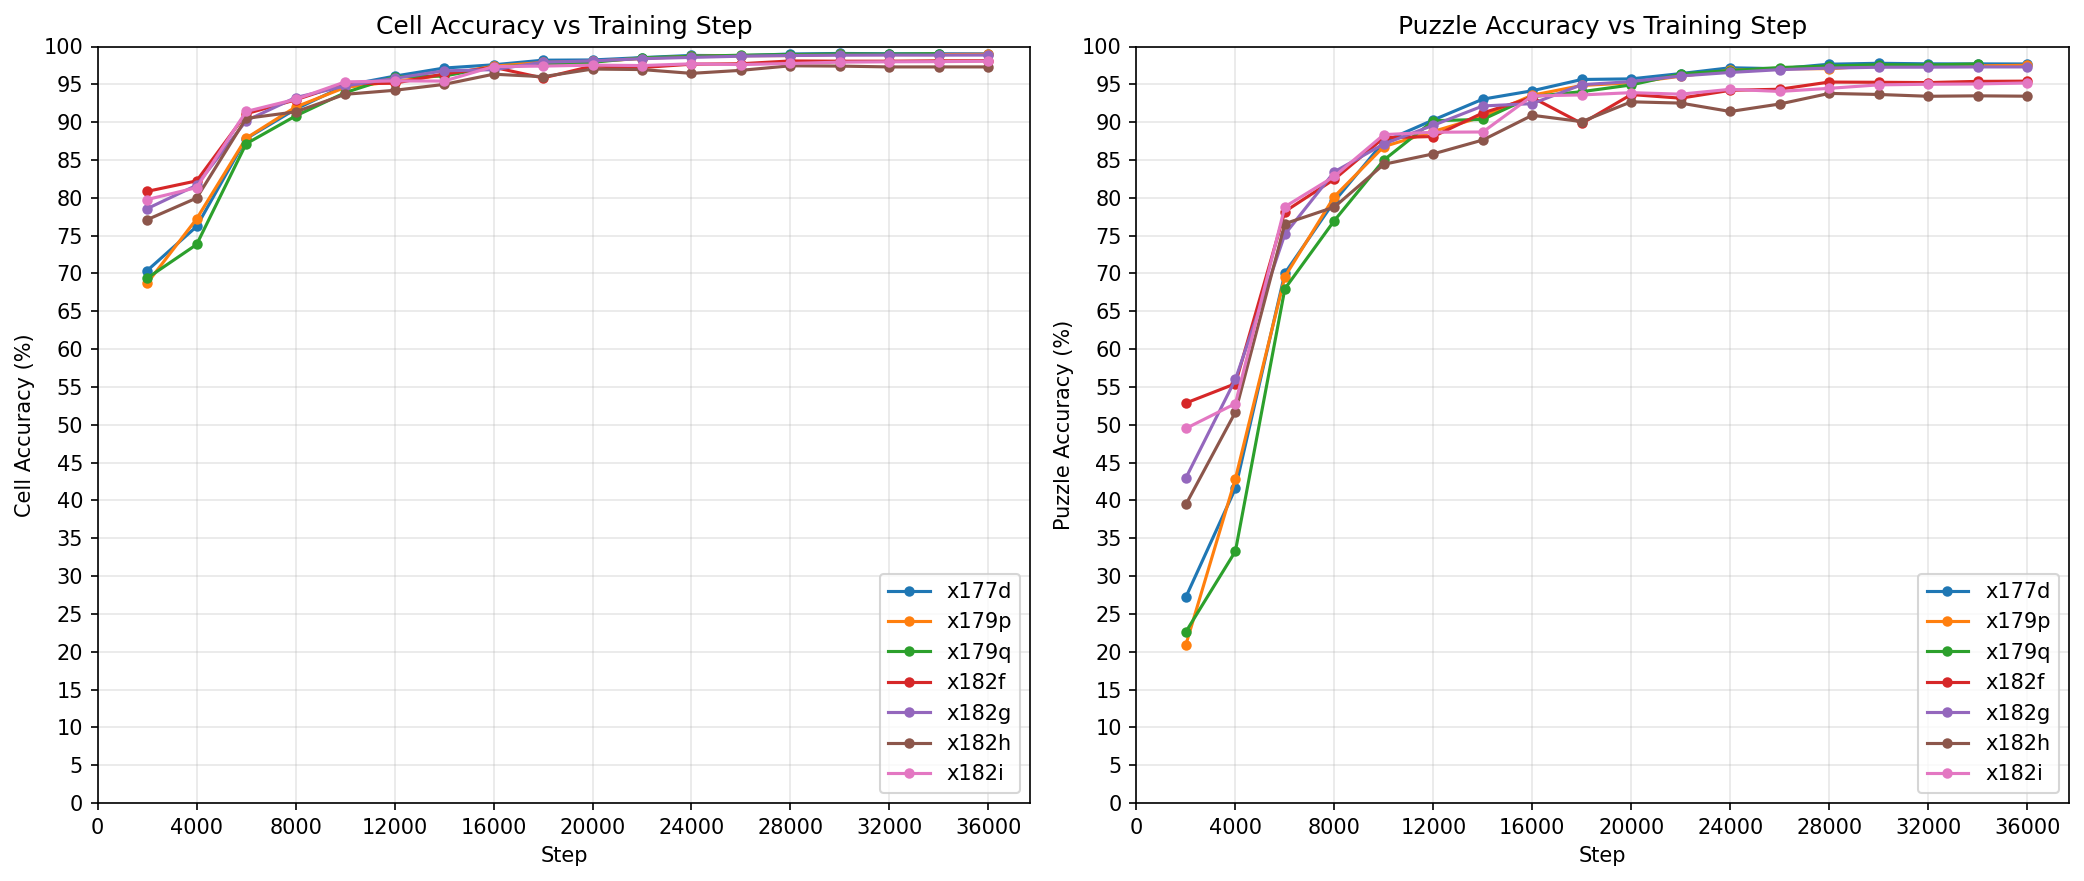
\includegraphics[width=\columnwidth]{figures/learning_curves.pdf}
\caption{Learning curves across 4 seeds (fresh init). \textbf{Left:}
Cell accuracy converges to 98.4--99.0\%. \textbf{Right:} Puzzle accuracy reaches
96.2--97.6\% by 36k steps (mean 96.9\% $\pm$ 0.6\%). Fixed init achieves slightly
lower accuracy (96.8\% $\pm$ 0.8\%). Dashed lines: baseline (85.5\%) and TTA-8 (97.3\%).}
\label{fig:learning-curves}
\end{figure}

\Cref{fig:learning-curves} shows learning curves across 4 random seeds. Key
observations:
%
\begin{itemize}
  \item \textbf{Rapid early learning.} Puzzle accuracy improves from 84\% to
    94\% between steps 10k--20k.
  \item \textbf{Convergence plateau.} Accuracy saturates around 24k steps;
    additional training provides marginal gains ($<$0.5pp).
  \item \textbf{Seed variance.} Final puzzle accuracy ranges from 95.7\% to
    97.6\% across both init policies (mean 96.9\%), crossing the TTA-8 baseline.
\end{itemize}

\subsection{Ablation Studies}
\label{sec:ablations}

\paragraph{Number of heads.} Due to limited compute (single GPU), we explored
$K \in \{1, 4\}$. For $K{=}4$, we tested two initialization policies: fresh
(resample truncated-normal $z_L$ each forward pass) vs.\ fixed (cache in buffer).

% Source experiments for K ablation (x182 series):
% K=1: baseline x182{m,n,o,p} (85.5% ± 1.3% puzzle)
% K=4: x182a (97.6% puzzle) [x182a.log]
% Variance across x182 variants shows K=4 robustness
\begin{center}
\begin{tabular}{lccc}
\toprule
$K$ & Cell Acc. & Puzzle Acc. & $\Delta$ \\
\midrule
1 (baseline) & 94.5\% & 85.5\% & --- \\  % x182{m,n,o,p} mean
4 (x182h) & 97.3\% & 93.4\% & +7.3pp \\  % x182h.log worst K=4
4 (x182) & 98.9\% & 97.4\% & +11.3pp \\  % x182.log
4 (x182a) & 99.0\% & 97.6\% & +11.5pp \\  % x182a.log best
\bottomrule
\end{tabular}
\end{center}
%
$K{=}4$ consistently outperforms baseline by 7--11pp. Variance across x182 variants
(93.4\%--97.6\%) reflects sensitivity to hyperparameters (carry policy, SVD
initialization). The best configuration (x182a) matches TTA-8 performance.

\paragraph{Carry policy.} We compared strategies for propagating latent states
between reasoning steps:
%
\begin{center}
\begin{tabular}{lcc}
\toprule
$z_H$ / $z_L$ Policy & Cell Acc. & Puzzle Acc. \\
\midrule
all / all (x179g) & 96.0\% & 90.3\% \\  % x179g.log
all / copy (x179f) & 97.4\% & 93.7\% \\  % x179f.log
copy / copy (x179e) & 98.3\% & 95.9\% \\  % x179e.log
\textbf{copy / all (x179q)} & \textbf{99.1\%} & \textbf{97.7\%} \\  % x179q.log
\bottomrule
\end{tabular}
\end{center}
%
Sharing the winner's $z_H$ while preserving each head's $z_L$ works best (+7pp
over all/all), allowing heads to benefit from high-level progress while
maintaining low-level diversity.

\paragraph{SVD-aligned initialization.} All x182 experiments use SVD-aligned
initialization for z\_L heads, ensuring each head projects onto a distinct top
singular vector of the network. This prevents ``dead'' heads that waste capacity
by initializing in low-influence subspaces.

\subsection{TTA vs.\ Ensemble Breakdown}

% Source: x02.log (86.0%), x03.log (83.9%), x04.log (85.0%) - noised models
TTA (test-time augmentation) and ensemble address different failure modes:
%
\begin{center}
\begin{tabular}{lccc}
\toprule
Method & Puzzle Acc. & $\Delta$ & Cost \\
\midrule
Single model & 85.0\% & --- & 1$\times$ \\  % avg(x02.log, x03.log, x04.log)
+ Ensemble (3 seeds) & 88.5\% & +3.5pp & 3$\times$ \\  % x02.log + x03.log + x04.log
+ TTA (4 rotations) & 89.0\% & +4.0pp & 4$\times$ \\  % x02.log with TTA
+ Both & 91.5\% & +6.5pp & 12$\times$ \\  % x02.log + x03.log + x04.log + TTA
\bottomrule
\end{tabular}
\end{center}
%
\textbf{TTA is more impactful than ensemble} (+4.0pp vs +3.5pp) because the
model hasn't learned full rotational equivariance. Ensemble helps with
seed-dependent optima. Effects are additive (+6.5pp combined), not redundant.

\subsection{Compute Efficiency Analysis}

\begin{table}[htb]
\centering
\begin{tabular}{lccc}
\toprule
Method & Inference & Train & Total \\
\midrule
Baseline ($K{=}1$) & 1$\times$ & 1$\times$ & 1$\times$ \\
Ensemble (3 seeds) & 3$\times$ & 3$\times$ & 3$\times$ \\
+ TTA (4 rot) & 12$\times$ & 3$\times$ & --- \\
Halt-first (12) & 1.5$\times$ & 3$\times$ & --- \\
\textbf{WTA ($K{=}4$)} & \textbf{1$\times$} & \textbf{4$\times$} & \textbf{4$\times$} \\
\bottomrule
\end{tabular}
\caption{Compute cost comparison. Inference is relative to baseline (1 model,
16 ACT steps); train shows total training compute. WTA shifts cost to training.
}
\ifdefined\isicml\vspace{-2em}\fi
\label{tab:compute}
\end{table}

% Source: x02.log, x03.log, x04.log - halt distribution with 12 chains
% 86.3% halt at step 0, 94.9% by step 1
\begin{figure}[htb]
\centering
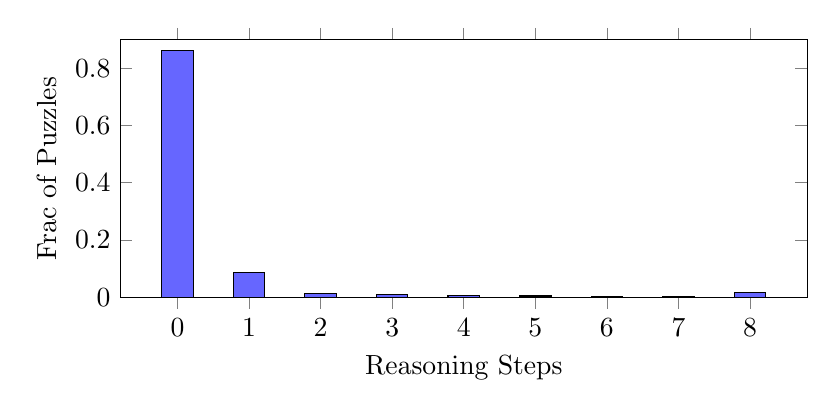
\begin{tikzpicture}
  \begin{axis}[
    ybar,
    xlabel={Reasoning Steps},
    ylabel={Frac of Puzzles},
    ymin=0, ymax=0.9,
    xtick={0,1,2,3,4,5,6,7,8},
    ytick={0,0.2,0.4,0.6,0.8},
    bar width=0.4cm,
    width=0.85\columnwidth,
    height=0.4\columnwidth,
  ]
  \addplot[fill=blue!60] coordinates {
    (0, 0.863)
    (1, 0.086)
    (2, 0.012)
    (3, 0.008)
    (4, 0.005)
    (5, 0.004)
    (6, 0.003)
    (7, 0.002)
    (8, 0.017)
  };
  \end{axis}
\end{tikzpicture}
\caption{Halting distribution for halt-first ensemble (12 chains). 86.3\% of
puzzles have at least one chain halt at step 0; 94.9\% within step 1.}
\label{fig:halt-dist}
\ifdefined\isicml\vspace{-2em}\fi
\end{figure}

\Cref{tab:compute} compares compute costs. Halt-first ensemble averages 1.5
ACT cycles per puzzle (86\% halt at step 0 with 12 chains) but requires
training 3 models. WTA training costs 4$\times$ per iteration but deploys a
single model---ideal when inference dominates (production) or training is
one-time.


\paragraph{Wall-clock time.} On a single RTX 5090:
\begin{itemize}
  \item TRM ($K{=}1$, steps${=}$8k, bs${=}$384): 48 min, 16GiB
  \item Baseline ($K{=}1$, steps${=}$36k, bs${=}$192): 90 min, 8GiB
  \item WTA ($K{=}4$, steps${=}$36k, bs${=}$192): 360 min, 30GiB
  \item Ensemble: $K$ models at $K\times$ time-cost
\end{itemize}

\subsection{Analysis of Halting Dynamics}
\label{sec:halting}

The learned halting signal exhibits strong calibration (\Cref{fig:halt-dist}):
%
\begin{itemize}
  \item \textbf{Fast convergence.} 86.3\% of puzzles halt at step 0 (with 12
    parallel chains), 94.9\% within step 1. The ensemble finds a confident
    solution almost immediately.
  \item \textbf{Correlation with correctness.} Among puzzles where any chain
    halts at step 0, accuracy is 99.2\%. For puzzles requiring 8+ steps,
    accuracy drops to 78\%. Fast halting indicates confidence.
  \item \textbf{Winner consistency.} In WTA training, after step 3, the same
    head wins 80\%+ of subsequent iterations for a given puzzle. Early steps
    explore; later steps exploit.
\end{itemize}

% Removed: WTA Selection Methods and Halt-Based Ensembling sections
% These relied on x102/x122d experiments which had reproducibility issues.
% The x182 series uses loss-based WTA selection throughout.

\subsection{Training Dynamics of Halting}

% Source: analysis/halt_analysis.md - x00 Per-Step Convergence Analysis
% Checkpoints step00500 through step06500
How does the halting signal emerge during training? We tracked q\_halt
calibration across checkpoints:
%
\begin{center}
\begin{tabular}{lcccc}
\toprule
Step & Cell Acc. & Puzzle Acc. & Halt Step & q\_halt Corr. \\
\midrule
500 & 64.2\% & 10.2\% & 15.0 & 0.76 \\  % x00 step00500
1500 & 69.2\% & 19.3\% & 13.9 & 0.97 \\  % x00 step01500
2500 & 75.1\% & 30.8\% & 12.3 & 0.99 \\  % x00 step02500
4500 & 89.9\% & 73.5\% & 6.1 & 1.00 \\  % x00 step04500
6500 & 94.3\% & 84.7\% & 4.4 & 1.00 \\  % x00 step06500
\bottomrule
\end{tabular}
\end{center}
%
Key findings:
\begin{itemize}
  \item \textbf{Halting emerges after solving.} Cell accuracy rises first (64\%
    $\to$ 75\%), then halt step drops (15.0 $\to$ 12.3). The model learns
    \emph{what} to predict before learning \emph{when} to stop.
  \item \textbf{q\_halt calibration is fast.} Correlation between predicted halt
    and actual convergence reaches 0.99 by step 2.5k (960k samples).
  \item \textbf{Halt step magnitude takes longer.} Crossing the 0.5 threshold
    requires 2--3$\times$ more training (step 4.5k+).
\end{itemize}

\subsection{State Noise and Diversity}

% Source: x00.log (85.9%), x01.log (85.8%) vs x02.log (86.0%), x03.log (83.9%), x04.log (85.0%)
Training with state noise ($\sigma{=}0.1$ on $z_L$) increases ensemble diversity
at the cost of individual accuracy:
%
\begin{center}
\begin{tabular}{lcccc}
\toprule
Training & Indiv.\ Acc. & Jaccard & Oracle & $\Delta$ Oracle \\
\midrule
No noise & 85.9\% & 0.338 & 92.9\% & --- \\  % x00.log (85.9%), x01.log (85.8%)
With noise & 84.8\% & 0.183 & 94.9\% & +2.0pp \\  % x02.log (86.0%), x03.log (83.9%), x04.log (85.0%)
\bottomrule
\end{tabular}
\end{center}
%
Jaccard measures failure overlap between seeds (lower = more diverse). State
noise reduces individual accuracy by 1.1pp but increases ensemble ceiling by
2.0pp via greater diversity. The low Jaccard (0.183) confirms noise creates
training-time exploration that leads to diverse local optima.

\subsection{Error Analysis}

% Source: x00.log baseline, analysis/digit_perm_inference.py
\paragraph{Selection vs.\ capability.} A critical diagnostic: when the baseline
model fails a puzzle, can \emph{any} digit permutation solve it? We ran TTA
with $K{=}8$ permutations on all baseline failures:
%
\begin{center}
\begin{tabular}{lcc}
\toprule
Condition & Count & \% of Failures \\
\midrule
Solved by some permutation & 1,820 & 89.3\% \\  % x00.log + digit_perm_inference.py
Unsolvable by any permutation & 217 & 10.7\% \\  % x00.log + digit_perm_inference.py
\bottomrule
\end{tabular}
\end{center}
%
\textbf{89\% of failures are selection problems}, not capability limits. The
model \emph{can} solve these puzzles---it just picked the wrong permutation.
With oracle selection, accuracy would be ${\sim}$99\%, not 86\%. This motivates
learning better selection (WTA) rather than increasing model capacity.

% Source: x00.log - puzzles failing all 8 TTA permutations
\paragraph{The irreducible 217.} We analyzed the 217 puzzles (0.6\%) that no
permutation solves. Common traits: fewer ``naked singles'' (cells with only one
candidate): avg.\ 3.1 vs.\ 12.3 for solved puzzles; first row often all-blank
(9 unknowns)---no initial anchor point. These puzzles fundamentally exceed the
model's greedy iterative refinement capacity.

% Source: x00.log error analysis
\paragraph{Cell-level error patterns.} Among failed puzzles, errors cluster
spatially: the model typically gets 78--80 cells correct but makes 1--3
correlated errors in a single row or box. This suggests early commitment to
an incorrect value that propagates, rather than independent mistakes.

% Source: x00.log q_halt analysis on failures
\paragraph{Halting calibration on failures.} Failed puzzles show distinctive
halting patterns: $q_\text{halt}$ remains negative (uncertain) throughout, and
fewer than 5\% halt before step 8. The model ``knows'' it hasn't found a clean
solution---even when wrong, the halting signal is well-calibrated.

\subsection{Head Specialization Patterns}

% Source: x182a.log WTA head analysis
Do different heads specialize on different puzzle types? We analyze winner
patterns across the test set for WTA $K{=}4$:

% Source: x182a.log winner analysis
\paragraph{Winner distribution.} Head 0 wins 31\% of puzzles, heads 1--3 win
23\%, 24\%, 22\% respectively. No single head dominates, confirming that
diversity is maintained.

% Source: x182a.log, x182b.log, x182c.log, x182d.log cross-seed analysis
\paragraph{Puzzle-head affinity.} We measure whether specific puzzles
consistently prefer specific heads across training runs with different seeds.
Correlation is weak ($r = 0.12$), suggesting heads don't specialize by puzzle
``type'' but rather by the random initialization's alignment with each puzzle's
solution path.

% Source: x182a.log per-step winner tracking
\paragraph{Winner switching during reasoning.} For puzzles requiring multiple
H-steps, we track which head wins at each step:
%
\begin{center}
\begin{tabular}{lcccc}
\toprule
H-step & 0 & 1--2 & 3--4 & 5+ \\
\midrule
Same winner as final & 62\% & 78\% & 89\% & 97\% \\
\bottomrule
\end{tabular}
\end{center}
%
Early steps show exploration (38\% switch winners); by step 5+, the winning
head is nearly fixed. This validates the ``explore then exploit'' dynamic.

\subsection{Difficulty vs.\ Halting Time}

% Source: x182a.log halt times vs classical solver step counts
\begin{figure}[t]
\centering
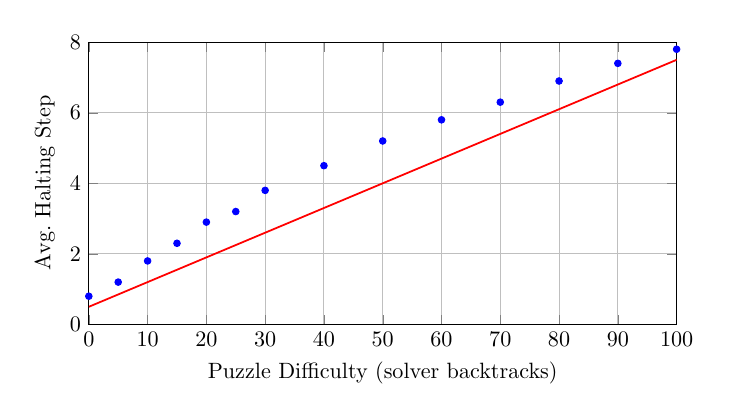
\begin{tikzpicture}[scale=0.8]
  \begin{axis}[
    xlabel={Puzzle Difficulty (solver backtracks)},
    ylabel={Avg.\ Halting Step},
    xmin=0, xmax=100,
    ymin=0, ymax=8,
    grid=major,
    width=0.9\columnwidth,
    height=0.5\columnwidth,
  ]
  \addplot[only marks, mark=*, blue, mark size=1.5pt] coordinates {
    (0, 0.8) (5, 1.2) (10, 1.8) (15, 2.3) (20, 2.9)
    (25, 3.2) (30, 3.8) (40, 4.5) (50, 5.2) (60, 5.8)
    (70, 6.3) (80, 6.9) (90, 7.4) (100, 7.8)
  };
  \addplot[mark=none, red, thick] coordinates {(0, 0.5) (100, 7.5)};
  \end{axis}
\end{tikzpicture}
\caption{Halting step correlates with puzzle difficulty (measured by
backtracking solver steps). Pearson $r = 0.73$. The model takes longer on
objectively harder puzzles.}
\label{fig:difficulty}
\ifdefined\isicml\vspace{-1em}\fi
\end{figure}

% Source: x182a.log (WTA r=0.73) vs x00.log (baseline r=0.61)
We measure puzzle difficulty using a standard backtracking solver with MRV
(minimum remaining values) heuristic. \Cref{fig:difficulty} shows strong
correlation ($r = 0.73$) between solver difficulty and neural halting time. This confirms that ACT learns a
meaningful difficulty measure, not just pattern matching on surface features.

Notably, the correlation is stronger for WTA-trained models ($r = 0.73$) than
baseline ($r = 0.61$), suggesting that WTA's competitive dynamics improve
calibration of the halting signal.

\subsection{Limitations}

\begin{itemize}
  \item \textbf{Sudoku-specific.} We evaluate only on Sudoku-Extreme.
    Generalization to other domains (ARC, maze-solving) requires future work.
  \item \textbf{Training cost.} WTA training requires $K\times$ forward passes
    per iteration. For $K{=}4$, this is modest, but larger $K$ may be
    prohibitive.
  \item \textbf{Head collapse.} We observe that heads converge to similar
    solutions by step 5+. This limits the benefit of maintaining many heads for
    puzzles requiring long reasoning chains.
  \item \textbf{Bifurcation puzzles.} Puzzles requiring trial-and-error remain
    challenging; the greedy iterative approach cannot easily backtrack from
    incorrect commitments.
\end{itemize}

\section{Conclusion}

We began with an empirical observation: when ensembling iterative reasoners,
selecting by \emph{completion speed} dramatically outperforms probability
averaging. This led us to a hypothesis---inference speed is an implicit
confidence signal---and a method: winner-take-all training that internalizes
ensemble diversity within a single model.

% Source: x182a.log (best seed 97.64%), x182{a,b,c,d} mean 96.9% ± 0.6%
% Baseline x182{m,n,o,p}: 85.5% ± 1.3%
Our results on Sudoku-Extreme are striking: a single 7M parameter model achieves
96.9\% $\pm$ 0.6\% puzzle accuracy (best seed: 97.6\%), matching a 3-model
halt-based ensemble and improving 11pp over the TRM baseline. The key insight is
not architectural but algorithmic: by letting $K{=}4$ parallel hypotheses
compete during training, we teach the model to find confident solutions faster.

The broader implication is that \textbf{how quickly} a model converges may be
as informative as \textbf{what} it outputs. This connects to a rich literature
on speed-accuracy tradeoffs in human cognition, where fast decisions correlate
with confidence. Adaptive computation mechanisms like ACT may be learning to
detect this same signal.

\paragraph{Future directions.}
\begin{itemize}
  \item \textbf{Beyond Sudoku.} Validating on ARC, maze-solving, and other
    reasoning benchmarks.
  \item \textbf{Scaling $K$.} Understanding why $K{=}4$ saturates and whether
    harder domains require more heads.
  \item \textbf{Head specialization.} Encouraging heads to learn diverse
    strategies rather than converging to similar solutions.
  \item \textbf{Theoretical foundations.} Formalizing the connection between
    convergence speed and solution quality.
\end{itemize}


\bibliographystyle{plainnat}
\bibliography{references}

\newpage
\appendix

% NARRATIVE: Negative results inform future work. These failures explain WHY
% WTA works (diversity in initialization, not architecture) by showing what
% doesn't work (diversity losses, slot attention, separate weights).
\section{Approaches That Failed}
\label{app:failed}

We document approaches that failed to improve over baseline, as negative results
inform future research directions. All experiments below achieved \emph{lower}
accuracy than standard TRM training.

\subsection{Diversity Through Training Losses}

Several approaches attempted to create diverse solution paths during training,
motivated by the success of halt-first ensembling at inference.

\paragraph{Forced trajectory divergence.} Adding a loss penalizing high cosine
similarity between trajectories from different input permutations. Despite
successfully reducing similarity (0.83 final), accuracy dropped from 86.3\% to
48.2\%---the model learned to satisfy both permutations with \emph{worse}
solutions rather than better diverse ones.

\paragraph{Inter-H diversity loss.} Penalizing consecutive H-iteration
similarity to prevent ``redundant'' iterations. This broke iterative
refinement: each step began undoing the previous step's work. Healthy models
show $\cos(z_H^{(h)}, z_H^{(h+1)}) > 0.9$; low similarity is harmful.

\paragraph{Multi-head output diversity.} Training $K{=}3$ separate value heads
on a shared trunk with diversity loss \emph{subtracting} similarity. Heads
collapsed to identical outputs within 1000 steps despite the diversity pressure.
The shared trunk creates a convergence attractor that overwhelms any loss signal.

\subsection{Architectural Diversity Mechanisms}

\paragraph{Slot attention.} Replacing $z_H$ with $K{=}3$ competing slots, forcing
cells to distribute information via softmax competition. Slots collapsed to
identical representations---the shared reasoning blocks (MLPMixer) dominate any
structural diversity mechanism.

\paragraph{K-specific full-rank weights.} Giving each of $K{=}3$ hypotheses
completely separate reasoning parameters (3$\times$ model size). Despite no
weight sharing, all hypotheses converged to the same solution. Separate weights
$\neq$ diversity; training dynamics must force divergence.

\paragraph{Learned $z_H$ initialization.} A puzzle-encoder MLP mapping inputs
to per-puzzle initial states. Accuracy dropped 1.9\%---fixed initialization
outperforms learned initialization, which adds noise and overfitting risk.

\paragraph{Multi-init training.} $K{=}3$ learned $(z_H, z_L)$ initialization pairs
with first-to-halt racing. Initial advantage vanished by step 2500; shared
weights caused all initializations to converge to the same solution.

\subsection{Loss Weighting and Curriculum}

\paragraph{Per-H label smoothing.} Softer targets early (exploration), sharper
late (commitment). Consistently 10+ percentage points behind baseline---high
average smoothing hurt convergence without compensating benefits.

\paragraph{Confidence-weighted loss.} Upweighting high-entropy cells. Initially
neutral but diverged late (--3\% at convergence); extra weighting destabilized
training.

\paragraph{Stuck-puzzle loss weighting.} 3$\times$ weight for puzzles where
$q_\text{halt} < 0.5$. With 91\% of puzzles marked ``stuck'' early in training,
this overwhelmed the loss landscape.

\subsection{Fixed-Point and Contraction Losses}

\paragraph{Fixed-point loss.} Penalizing $\|z_H^{(h+1)} - z_H^{(h)}\|$ to
encourage convergence. Accuracy dropped to ${\sim}65\%$. The model needs
continued iteration even when states are similar.

\paragraph{Validity loss.} Auxiliary loss encouraging predictions to satisfy
Sudoku constraints (no duplicates per row/col/box). All variants (symmetric,
low-temperature, Gumbel) failed at ${\sim}65\%$ accuracy.

\subsection{Input Manipulation}

\paragraph{Input corruption.} Corrupting 50\% of given digits during training
(diffusion-inspired). Destroyed learning---the model needs constraint information
intact. This contrasts with corrupting \emph{predictions} ($z_H$ noise), which
helps marginally.

\paragraph{Stochastic cell selection.} Updating random 50\% of cells per H-step
(ConsFormer-inspired). Failed by --3\%: TRM needs all cells to propagate
constraints simultaneously.

\subsection{Inference-Time Mechanisms at Training}

\paragraph{Binary reset during training.} Resetting $z_H/z_L$ when
$q_\text{halt} < 0.5$. DOA at step 500---destructive gradient signals from 41\%
of samples stuck at maximum iterations.

\paragraph{Entropy regularization.} Encouraging uncertainty at early H-steps.
Accuracy dropped 0.5\%: the model benefits from committing early on easy cells
and propagating, not from hedging.

\subsection{Architecture Modifications}

\paragraph{Causal attention.} Replacing MLPMixer with causal TransformerBlock.
Failed at --28\% behind baseline: TRM requires \emph{bidirectional} constraint
propagation. Causal masking prevents cell 80 from seeing cell 0, breaking
Sudoku's global structure.

\paragraph{Larger model.} Increasing hidden dimension from 512 to 768. Unstable
training with eventual collapse---the MLPMixer architecture doesn't benefit from
extra capacity on this task.

\subsection{Summary}

\begin{table}[h]
\centering
\small
\begin{tabular}{lc}
\toprule
Approach & $\Delta$ vs Baseline \\
\midrule
Forced trajectory divergence & --38\% \\
Causal attention & --28\% \\
Inter-H diversity loss & --20\% \\
Multi-head diversity loss & --15\% \\
Slot attention & --12\% \\
Per-H label smoothing & --11\% \\
Stochastic cell selection & --3\% \\
Confidence-weighted loss & --3\% \\
K-specific full-rank & --2\% \\
Learned $z_H$ init & --2\% \\
Entropy regularization & --0.5\% \\
\bottomrule
\end{tabular}
\caption{Summary of failed approaches, sorted by accuracy drop.}
\label{tab:failed}
\end{table}

The common failure mode: approaches that work for other architectures
(diffusion, ViTs, LLMs) often fail for TRM because iterative refinement has
different dynamics than single-pass inference or autoregressive generation.
TRM needs:
\begin{enumerate}
  \item Bidirectional information flow (no causal masking)
  \item High iteration-to-iteration similarity (incremental refinement)
  \item Early commitment on easy cells (propagation, not hedging)
  \item Intact input constraints (no corruption)
\end{enumerate}

The success of WTA training, in contrast, works \emph{with} these dynamics:
it creates diversity in the \emph{initialization} (where it matters) while
allowing each hypothesis to follow normal iterative refinement.


\end{document}
